\section*{Results}

\begin{center}
    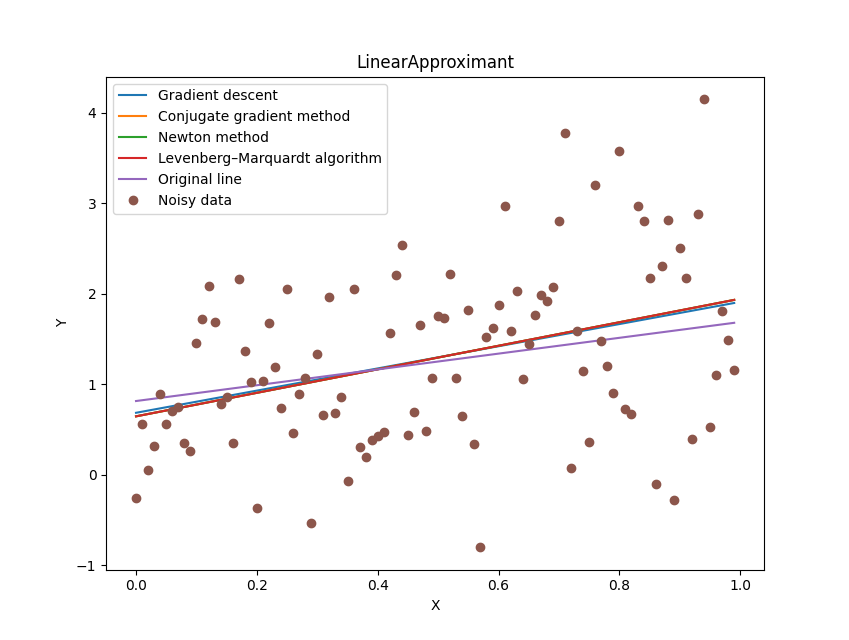
\includegraphics[width=0.7\textwidth]{../results/linear.png}
    \captionof{figure}{Linear approximant}
\end{center}

\begin{center}
    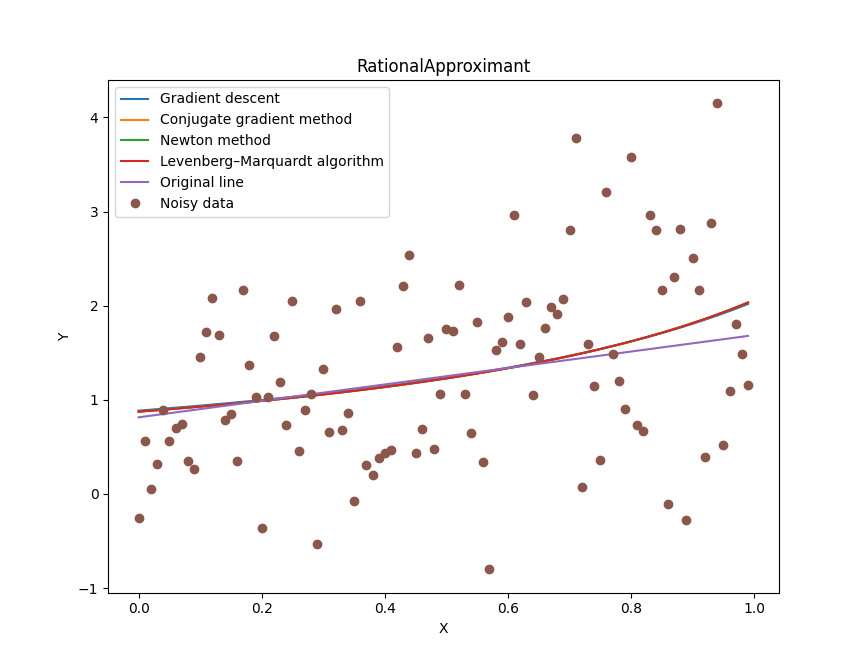
\includegraphics[width=0.7\textwidth]{../results/rational.png}
    \captionof{figure}{Rational approximant}
\end{center}

For both approximants all optimizers finds similar sollutions, although the particular found sollution for rational approximant sdepends 
on initial values.


\begin{table*}[h!]
    \begin{center}
        \caption{Optimization results for direct methods}
        \label{table:direct-methods}
        \begin{tabular}{|c|c|c|c|c|}
            \textbf{Algorithm} & \textbf{$a, b$} & \textbf{$(\hat{y} - y)^2$} & \textbf{Evaluations} & \textbf{Iterations}\\
            \hline
            Real & (0.87, 0.81) & 82.36 & &\\
            Brute-force & (1.3004, 0.6455) & 80.6719 & 2253001 & 2253001 \\
            Gauss & (1.3028, 0.6434) & 80.6719 & 864 & 800 \\
            Nelder-Mead & (1.3000, 0.6448) & 80.6719 & 117 & 60
        \end{tabular}
    \end{center}
\end{table*}

\begin{table*}[h!]
    \begin{center}
        \caption{Optimization results for first- and second-order methods}
        \label{table:high-order-methods}
        \begin{tabular}{|c|c|c|c|c|}
            \textbf{Algorithm} & \textbf{$a, b$} & \textbf{$(\hat{y} - y)^2$} & \textbf{Evaluations} & \textbf{Iterations}\\
            \hline
            Real & (0.87, 0.81) & 82.36 & &\\
            Gradient descent & (1.299, 0.6555) & 80.7719 & 183 & 183 \\
            Conjugate gradient descent & (1.3003, 0.6444) & 80.6719 & 18 & 3 \\
            Newton's method & (1.3003, 0.6444) & 80.6719 & 18 & 4 \\
            Levenberg-Marquardt algorithm & (1.3003, 0.6444) & 80.6719 & 6 & 6 \\
        \end{tabular}
    \end{center}
\end{table*}

From tables \ref{table:direct-methods}, \ref{table:high-order-methods} it can be seen that first and second order methods
require less iterations and function evaluations for finding sollution with the same precision. 

The best results in terms of iterations are shown by Conjuagate gradient descent method, Newton's method requires slighly more iterations for linear approximant optimization. On the other hand, LMA requires the least number of function evaluations.

The worst results in terms of iterations and function evaluations are shown by Gradient descent - the number of requred iteration is even higher than for direct Nelder-Mead method, as well as that
conducted experiments showed that it is more sensitive for paremeters for proper convergence.